\section{One Material}
For the first test problem we used a single material with  upscattering throughout a 20 by 20 domain with a constant source. We used cross sections for the seven group moderator material in the C5G7 benchmark problem. \cite{C5G7}.  
The problems were run on a single processor of a MacBook Pro. 
\begin{center}
    \begin{tabular}{|c|c|c|}
    \hline
    & Runtime (s) & GS Iterations \\
    \hline
    TG-NDA & 5465.00732 & 9 \\
    NDA & 14513.23 & 31 \\
    \hline
    \end{tabular}
\end{center}
The two-grid method provides a considerable acceleration of the Gauss-Seidel method. While when using TG-NDA each iteration takes slightly longer as the correction term must be calculated, it more than makes up for it with a considerable decrease in the number of iterations necessary to reach convergence. 

Importantly, the accleration in convergence came at no cost to accuracy. As can be seen in the figure below, the NDA and TG-NDA solutions have the same values (up to tolerance). In the interest of space, we only show the results from the highest energy group, but the NDA/TG-NDA agreement held for all energy groups in our test problems. 
\begin{figure}[H]
\centering
\begin{subfigure}{.5\textwidth}
  \centering
  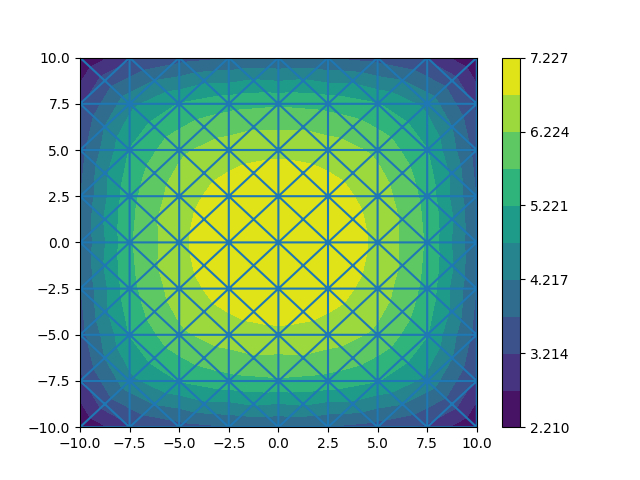
\includegraphics[width=\linewidth]{fig/nda_c5g7mod_scalar_flux_group0.png}
  \caption{Highest Energy Group, NDA}
  \label{fig:NDA-Mod}
\end{subfigure}%
\begin{subfigure}{.5\textwidth}
  \centering
  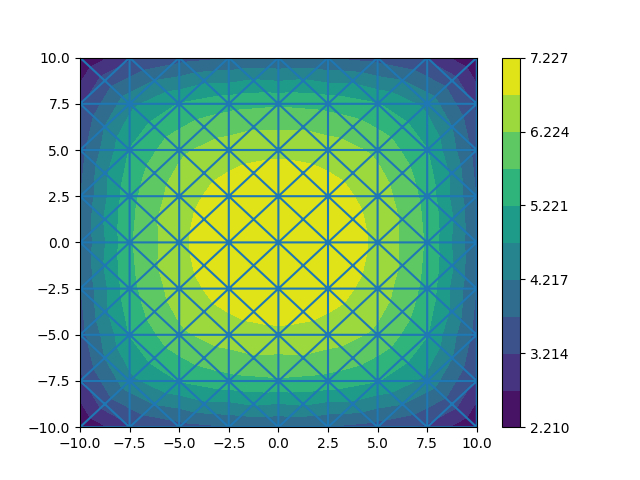
\includegraphics[width=\linewidth]{fig/tgnda_c5g7mod_scalar_flux_group0.png}
  \caption{Highest Energy Group, TG-NDA}
  \label{fig:TG-NDA-Mod}
\end{subfigure}
\caption{Comparison of NDA/TG-NDA in Flux Value for One Material Problem}
\label{fig:Moderator}
\end{figure}
\section{Two Materials}
The second problem consists of two materials in a concentric geometry with a box source in the center. The first material, located in the center and outer layer, is the C5G7 moderator material used above and the second material has the same total cross sections and pattern of upscatter, but with higher absorption and lower total scattering. Both materials have seven groups. There is a box source in the center that emits 70\% in the highest energy group, 20\% in the second highest, and 10\% in the third.
\begin{figure}[H]
    \centering
    
\includegraphics[width=.3\textwidth]{fig/Geometry.png}
    \caption{Geometry of Two-Material Test Problem}
    \label{fig:test_geometry}
\end{figure}

\begin{center}
    \begin{tabular}{|c|c|c|}
    \hline
    & Runtime (s) & GS Iterations \\
    \hline
    TG-NDA & 4221.92 & 8 \\
    NDA & 10381.52 & 25 \\
    \hline
    \end{tabular}
\end{center}

Again, TG-NDA showed a significant improvement over the unaccelerated Gauss Seidel, taking roughly a third of the number of iterations. Again, NDA and TG-NDA agree in terms of flux values. Here we also only show results for the highest energy group. 
\begin{figure}[H]
\centering
\begin{subfigure}{.5\textwidth}
  \centering
  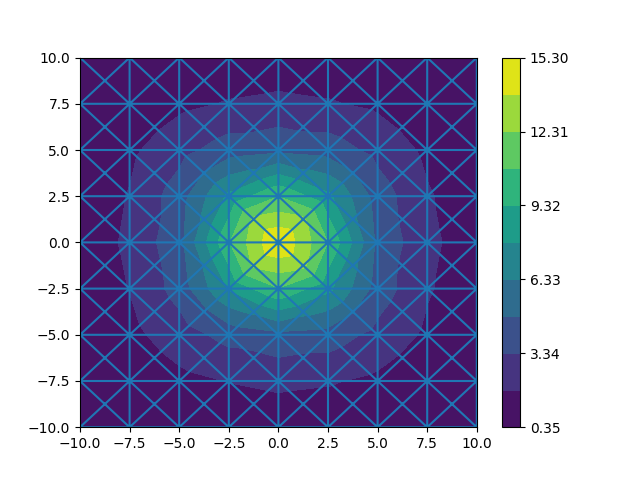
\includegraphics[width=\linewidth]{fig/nda_iron-water_scalar_flux_group0.png}
  \caption{Highest Energy Group, NDA}
  \label{fig:NDA-Mod}
\end{subfigure}%
\begin{subfigure}{.5\textwidth}
  \centering
  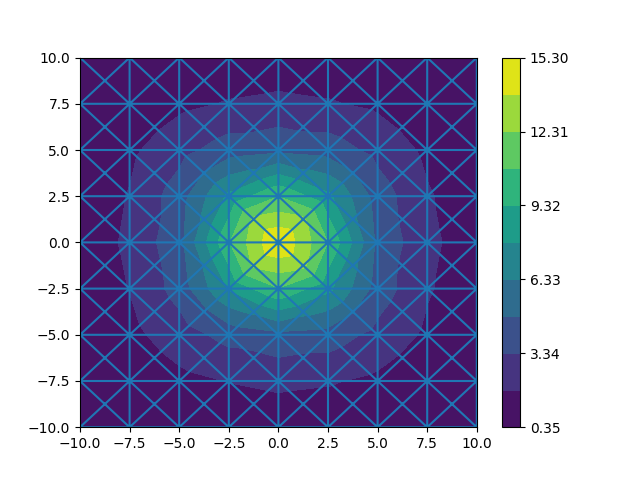
\includegraphics[width=\linewidth]{fig/tgnda_iron-water_scalar_flux_group0.png}
  \caption{Highest Energy Group, TG-NDA}
  \label{fig:TG-NDA-Mod}
\end{subfigure}
\caption{Comparison of NDA/TG-NDA in Flux Value for Two Material Problem}
\label{fig:Moderator}
\end{figure}

\section{Reproducibility}
The code used to run these experiments is hosted online at \\ www.github.com/mzweig/gallo. The version used is tagged as masters-thesis. The geometry inputs \texttt{origin-centered10} and material input \texttt{c5g7mod} were used for the first test problem, and the geometry input \texttt{iron-water10} and material input \texttt{mod-water} were used for the second problem. 